\chapter{Implementation \& Version Control}
\label{ch:implementation}

Design documents do not run; code does. Implementation translates design into executable software while managing complexity, collaboration, and change. Version control is the safety net that makes collaborative implementation possible at scale.

\section{From Design to Code}

Good implementation respects design intent while adapting to discovered realities. Key practices include:

\begin{itemize}
    \item \textbf{Coding standards} --- naming, formatting, and idiom conventions that make code look like it was written by one person. Enforced by linters and formatters.
    \item \textbf{Defensive programming} --- validate inputs, fail fast with clear messages, handle edge cases explicitly.
    \item \textbf{Reuse} --- prefer well-tested libraries and frameworks over reinventing the wheel; manage dependencies explicitly.
    \item \textbf{Continuous integration} --- integrate to mainline frequently (at least daily) to avoid big-bang merge pain.
\end{itemize}

\begin{lstlisting}[language=Java,caption={Defensive programming: fail fast with preconditions.}]
public final class Enrollment {
    private final Student student;
    private final Course course;
    public Enrollment(Student s, Course c) {
        if (s == null || c == null) throw new IllegalArgumentException("null arg");
        if (c.isFull()) throw new IllegalStateException("course full: " + c.getCode());
        this.student = s; this.course = c;
    }
}
\end{lstlisting}

\section{Version Control Fundamentals}

Version control tracks every change, who made it, and why. It enables branching (parallel lines of work), merging (combining branches), tagging (marking releases), and reverting (undoing mistakes). Centralised systems (SVN) have a single server; distributed systems (Git) give every developer a full repository, enabling offline work and flexible workflows.

\subsection{Git Core Concepts}

\begin{itemize}
    \item \textbf{Repository} --- the \texttt{.git} directory storing all history as a DAG of commits.
    \item \textbf{Commit} --- a snapshot identified by a SHA-1 hash, with a message explaining the change.
    \item \textbf{Branch} --- a movable pointer to a commit; cheap and disposable.
    \item \textbf{Remote} --- a shared repository (e.g., GitHub) that branches synchronise with via \texttt{push}/\texttt{fetch}.
    \item \textbf{Staging area (index)} --- where you assemble the next commit with \texttt{git add}.
\end{itemize}

\begin{figure}[h]
\centering
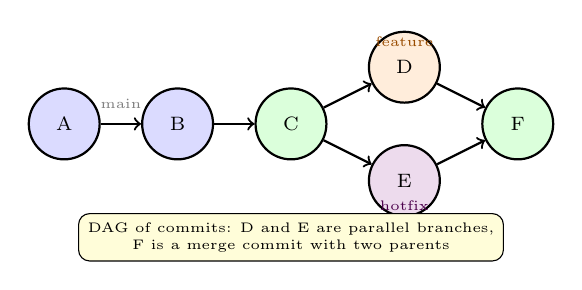
\begin{tikzpicture}[scale=0.72, every node/.style={font=\scriptsize}]
  \tikzstyle{c}=[draw,circle,fill=blue!14,minimum size=0.9cm,thick]
  \node[c] (a) at (0,0) {A};
  \node[c] (b) at (2,0) {B};
  \node[c,fill=green!14] (c) at (4,0) {C};
  \node[c,fill=orange!14] (d) at (6,1.0) {D};
  \node[c,fill=violet!14] (e) at (6,-1.0) {E};
  \node[c,fill=green!14] (f) at (8,0) {F};
  \draw[->,thick] (a) -- (b); \draw[->,thick] (b) -- (c);
  \draw[->,thick] (c) -- (d); \draw[->,thick] (c) -- (e);
  \draw[->,thick] (d) -- (f); \draw[->,thick] (e) -- (f);
  \node[draw,fill=yellow!15,rounded corners,font=\tiny,align=center] at (4,-2.0) {DAG of commits: D and E are parallel branches,\\F is a merge commit with two parents};
  \node[font=\tiny,gray] at (1,0.35) {main};
  \node[font=\tiny,orange!60!black] at (6,1.45) {feature};
  \node[font=\tiny,violet!60!black] at (6,-1.45) {hotfix};
\end{tikzpicture}
\caption{Git history as a directed acyclic graph -- branches diverge and merge; every commit has a parent (merge commits have two).}
\end{figure}

\section{Branching Workflows}

\subsection{Git Flow}

Git Flow (Vincent Driessen) structures branches by purpose:

\begin{itemize}
    \item \texttt{main} --- production-ready code; every commit is a release.
    \item \texttt{develop} --- integration branch for the next release.
    \item \texttt{feature/*} --- new features branched from \texttt{develop}, merged back when done.
    \item \texttt{release/*} --- stabilisation (bug fixes, version bumps) branched from \texttt{develop}.
    \item \texttt{hotfix/*} --- urgent production fixes branched from \texttt{main}, merged to both \texttt{main} and \texttt{develop}.
\end{itemize}

\begin{figure}[h]
\centering
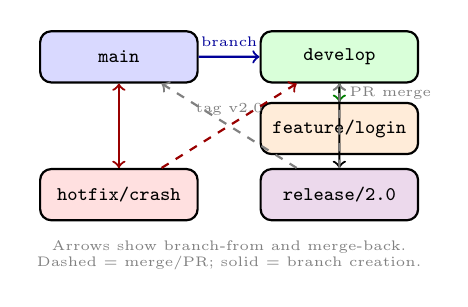
\begin{tikzpicture}[scale=0.70, every node/.style={font=\scriptsize}]
  \tikzstyle{br}=[draw,rounded corners,minimum width=2.0cm,minimum height=0.65cm,align=center,thick]
  \node[br,fill=blue!15] (main) at (0,2.4) {\texttt{main}};
  \node[br,fill=green!15] (dev) at (4,2.4) {\texttt{develop}};
  \node[br,fill=orange!15] (feat) at (4,1.1) {\texttt{feature/login}};
  \node[br,fill=violet!15] (rel) at (4,-0.1) {\texttt{release/2.0}};
  \node[br,fill=red!12] (hot) at (0,-0.1) {\texttt{hotfix/crash}};
  \draw[->,thick,blue!60!black] (main) -- (dev) node[midway,above,font=\tiny] {branch};
  \draw[->,thick,green!50!black] (dev) -- (feat);
  \draw[->,thick,dashed,gray] (feat) -- (dev) node[midway,right,font=\tiny] {PR merge};
  \draw[->,thick] (dev) -- (rel);
  \draw[->,thick,dashed,gray] (rel) -- (main) node[midway,above,font=\tiny] {tag v2.0};
  \draw[->,thick,dashed,gray] (rel) -- (dev);
  \draw[->,thick,red!60!black] (main) -- (hot);
  \draw[->,thick,dashed,red!60!black] (hot) -- (main);
  \draw[->,thick,dashed,red!60!black] (hot) -- (dev);
  \node[font=\tiny,gray,align=center] at (2,-1.2) {Arrows show branch-from and merge-back.\\Dashed = merge/PR; solid = branch creation.};
\end{tikzpicture}
\caption{Git Flow branching model -- disciplined separation of features, releases, and hotfixes. Many teams now prefer the simpler GitHub Flow (feature branches directly to main with CI).}
\end{figure}

\subsection{GitHub Flow and Trunk-Based Development}

GitHub Flow is lighter: every change is a feature branch off \texttt{main}, reviewed via pull request (PR), CI-tested, then merged. Trunk-based development goes further: developers commit small changes directly to \texttt{main} (or very short-lived branches $<$1~day), using feature flags to hide incomplete work. Trunk-based development requires excellent CI and test coverage but yields the fastest feedback.


\section{Build Systems and Dependency Management}

Modern projects automate compilation, testing, and packaging via build tools: \texttt{make}, Gradle, Maven, npm, or Bazel. A reproducible build specifies exact dependency versions (lock files), runs in a clean environment (containers), and is triggered by every push via CI. Dependency management distinguishes direct from transitive dependencies; tools like Dependabot flag vulnerable transitive dependencies that would otherwise go unnoticed.

\begin{lstlisting}[language=Python,caption={Reproducible dependencies with pip-tools.}]
# requirements.in  (direct deps only)
requests==2.31.0
pydantic>=2.0
# Compile to requirements.txt with hashes:
#   pip-compile --generate-hashes requirements.in
\end{lstlisting}

\section{Handling Merge Conflicts}

Conflicts arise when two branches edit the same lines. Git marks conflicted regions with \texttt{<<<<<<<}, \texttt{=======}, \texttt{>>>>>>>}. Resolution requires understanding \emph{intent}, not just picking one side. Strategies include rebasing feature branches frequently onto \texttt{develop} to keep conflicts small, using \texttt{git rerere} to reuse past resolutions, and enabling merge queues to serialise concurrent merges safely.

\section{Code Review and Collaboration}

Pull requests are the collaboration hub: code is reviewed, discussed, CI runs automated checks, and only then is it merged. Effective reviews are small ($<$400~lines), focused, and kind. Automated checks (lint, test, security scan) should run before human review to avoid wasting reviewer time on style nits.

\begin{lstlisting}[language=Python,caption={Pre-commit checks save reviewer time.}]
# .pre-commit-config.yaml (excerpt)
repos:
  - repo: https://github.com/psf/black
    hooks: [{id: black}]
  - repo: https://github.com/pycqa/flake8
    hooks: [{id: flake8}]
# Run: pre-commit install && pre-commit run --all-files
\end{lstlisting}



\section{Reproducibility and Environment Management}

``Works on my machine'' is a perennial failure mode. Reproducibility requires pinning dependency versions, containerising the runtime (Docker), and documenting setup so a new developer can go from clone to passing tests in one command (\texttt{make bootstrap}). Lock files (\texttt{package-lock.json}, \texttt{requirements.txt} with hashes, \texttt{poetry.lock}) ensure every install resolves to identical artefacts; without them, transitive updates can break builds nondeterministically.

\begin{lstlisting}[language=Python,caption={One-command bootstrap for reproducibility.}]
# Makefile
bootstrap:
	pip install -r requirements.txt
	pre-commit install
	pytest -q
# New developer: git clone <url> && make bootstrap
\end{lstlisting}

Container-based development goes further: the CI image and the developer image are the same Dockerfile, so environment drift is eliminated. Docker multi-stage builds keep production images small by discarding build-time dependencies.

\section{Continuous Integration in Practice}

A CI pipeline triggers on every push: checkout $\to$ install deps $\to$ lint $\to$ unit test $\to$ build $\to$ (optional) deploy to staging. Fast feedback is critical---CI should complete in under 10~minutes, or developers stop waiting and context-switch. Techniques to keep CI fast include test parallelisation, caching, and splitting slow end-to-end tests into a nightly job separate from the per-push gate.

\begin{figure}[h]
\centering
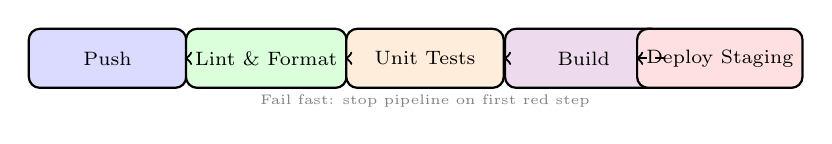
\begin{tikzpicture}[scale=0.72, every node/.style={font=\scriptsize}]
  \tikzstyle{cipstep}=[draw,rounded corners,minimum width=2.0cm,minimum height=0.75cm,align=center,thick]
  \node[cipstep,fill=blue!14] (a) at (0,0) {Push};
  \node[cipstep,fill=green!14] (b) at (2.8,0) {Lint \& Format};
  \node[cipstep,fill=orange!14] (c) at (5.6,0) {Unit Tests};
  \node[cipstep,fill=violet!14] (d) at (8.4,0) {Build};
  \node[cipstep,fill=red!12] (e) at (10.8,0) {Deploy Staging};
  \draw[->,thick] (a) -- (b); \draw[->,thick] (b) -- (c);
  \draw[->,thick] (c) -- (d); \draw[->,thick,dashed] (d) -- (e);
  \node[font=\tiny,gray] at (5.6,-0.75) {Fail fast: stop pipeline on first red step};
\end{tikzpicture}
\caption{Minimal CI pipeline -- every push is verified automatically; staging deploy is optional and gated on green tests.}
\end{figure}


\section{Semantic Versioning and Releases}

Semantic versioning (\texttt{MAJOR.MINOR.PATCH}) communicates breaking changes: MAJOR for incompatible API changes, MINOR for backward-compatible features, PATCH for backward-compatible fixes. Tags (\texttt{v2.1.0}) mark releases; release notes summarise changes by category. Automated release pipelines cut a tag, build artefacts, and publish to a registry without manual steps, reducing human error.

\section{Documentation as Code}

Architecture Decision Records (ADRs) capture why a decision was made, not just what was decided: context, options considered, decision, and consequences. Stored alongside code (e.g., \texttt{docs/adr/001-use-postgres.md}), ADRs prevent future developers from re-litigating settled debates or unknowingly violating constraints.

\section{Exercises}

\begin{exercise}
Explain why ``commit early, commit often'' with meaningful messages is better than one large commit at the end of a task. What makes a good commit message? Give a bad and a good example.
\end{exercise}

\begin{exercise}
A hotfix for a production crash must be delivered without including half-finished features on \texttt{develop}. Show the Git Flow branch sequence (commands or diagram) that achieves this and explain where the hotfix is merged.
\end{exercise}

\begin{exercise}
Compare Git Flow, GitHub Flow, and trunk-based development on three criteria: release cadence, team size suitability, and CI requirements. When would you choose each?
\end{exercise}

\begin{exercise}
A PR contains 1{,}200 lines across 15~files with no description. List four concrete problems this causes for reviewers and CI, and propose a better decomposition.
\end{exercise}

\begin{exercise}
Your team uses feature flags for trunk-based development. Explain how a flag lets you merge incomplete code to \texttt{main} safely, and describe two risks of long-lived flags that are never removed.
\end{exercise}
